%%%%%%%%%%%%
%% Please rename this main.tex file and the output PDF to
%% [lastname_firstname_graduationyear]
%% before submission.
%%%%%%%%%%%%

\documentclass[12pt]{caltech_thesis}
\usepackage[hyphens]{url}
%\usepackage{lipsum} %dummy content
\usepackage{graphicx}

%\usepackage{todonotes}

\usepackage{hyperref}



%% Tentative: newtx for better-looking Times
\usepackage[utf8]{inputenc}
\usepackage[T1]{fontenc}
\usepackage{newtxtext,newtxmath}

% Must use biblatex to produce the Published Contents and Contributions, per-chapter bibliography (if desired), etc.
\usepackage[
    backend=biber,natbib,
    % IMPORTANT: load a style suitable for your discipline
    style=authoryear
]{biblatex}

% Name of your .bib file(s)
\addbibresource{example.bib}
\addbibresource{ownpubs.bib}

\begin{document}

% Do remember to remove the square bracket!
\title{Development of Excitation Channel for KAGRA Photon Calibratior}
\author{Yu-Kuang Chu}

\degreeaward{Master of Science}                 % Degree to be awarded
\university{National Taiwan Normal University}    % Institution name
\address{Taipei, Taiwan}                     % Institution address
\unilogo{NTNU.png}                                 % Institution logo
\copyyear{2018}  % Year (of graduation) on diploma
\defenddate{[Exact Date]}          % Date of defense

\orcid{[Author ORCID]}

%% IMPORTANT: Select ONE of the rights statement below.
% \rightsstatement{All rights reserved\todo[size=\footnotesize]{Choose one from the choices in the source code!! And delete this \texttt{todo} when you're done that. :-)}}
% \rightsstatement{All rights reserved except where otherwise noted}
% \rightsstatement{Some rights reserved. This thesis is distributed under a [name license, e.g., ``Creative Commons Attribution-NonCommercial-ShareAlike License'']}

%%  If you'd like to remove the Caltech logo from your title page, simply remove the "[logo]" text from the maketitle command
\maketitle[logo]
%\maketitle

\begin{acknowledgements} 	 
  Thank everyone ~~~
\end{acknowledgements}

\begin{abstract}
   [This abstract must provide a succinct and informative condensation of your work. Candidates are welcome to prepare a lengthier abstract for inclusion in the dissertation, and provide a shorter one in the CaltechTHESIS record.]
\end{abstract}

%% Uncomment the `iknowhattodo' option to dismiss the instruction in the PDF.
\begin{publishedcontent}%[iknowwhattodo]
% List your publications and contributions here.
\nocite{Cahn:etal:2015,Cahn:etal:2016}
\end{publishedcontent}

\tableofcontents
\listoffigures
\listoftables
\printnomenclature

\mainmatter


\chapter{Introduction} 
\section{Introduction to Gravitational Wave}
\subsection{What is gravitational wave}
In the General Theory of Relativity proposed by Albert Einstein. The phenomenon caused by gravity in one frame can be interpreted as the result of curved spacetime.


Furthermore, the field equation of spacetime curvature allows wave-like solution similar to electromagnetic solution in Maxwell’s equation. In other words, the time-dependent local mass distribution can generate time-depend distortion of spacetime known as gravitational waves. These gravitational waves or the ripple of spacetime can propagate throughout the universe like electromagnetic waves.
	
However, the physical reality of gravitational wave is not so clear to everyone in the early days, even to Even Einstein himself~\cite{?}. The main problems is that there exist some gauge degree of freedom in the theory due to the arbitrariness of coordinate choices. We have to know whether the gravitational waves we found are just gauge waves (vibration of coordinate) or the wave can have some observable consequences. 

On of the most important observational evidence implying the existence of real gravitational waves is Hulse-Taylor pulsar.  
....
Finally, in 2015 September 14.
GW150914

\subsection{How to describe gravitational wave}
mathematics….

TTgauge
There is a very convenient gauge(coordinate) constrain, which is known as Traceless and Transverse gauge. 
for perturbation of wave like part metic over Schwarzschild background which represent Earth’s gravity.

How to generate gravitational wave
The source of electromagnetic wave is time-dependent electrical charge distribution.  Similarly, the source of gravitational wave is time-dependent mass(energy) distribution. Strictly speaking, the lowest order of mass multi-pole which can generate real gravitational waves is mass quadruple because we don’t have negative mass, while the electromagnet wave can be generate though time-dependent electrical dipole moment. The gravitational wave strain generated by mass quadruple can be approximately described by famous quadrupole formula:
(quadrupole formula)
According to our current understand of universe, there are several kinds of astrophysical gravitational wave sources, whose h(t) amplitude is large enough to be detected by current ground based laser interferometer, like advanced-LIGO, advanced-Virgo or KAGRA.
Compact Binary Coalescence 
BNS BBH
\subsection{How to detect Gravitational wave}
The interaction of detector and gravitational wave can have different interpretation due to different coordinate choice. It is quiet similar to that the magnetic force in one observational frame may be electric force in the other frame. However, practically, I would like to use the …….., which described in next section.


\section{Detection of Gravitation wave}

Interaction of GW wave when $\lambda_gw$ >> L of detector
Limit of Michelson IFO
IFO with dual-recycling and Fabry-Perot  arms.
Fucking Complex response
WE NEED Calibration Calibration Calibration



\section{Calibration and Reconstruction}

Calibration is always the fist step before we measure something by some device.
For example, to measure the weight of an apple, you should calibrate your scale by putting a “standard kilogram” on it. Then, you can either adjust the scale readout to be 1kg, or record the difference showed in scale readout, which may be used to reconstruct real weight of the apple. However, the spring constant of springs inside the scale could fluctuate due to temperature changes. To accurately measure the weight of the apple, we have to measure the calibration factor (scale readout when we put the standard mass on it.) when we measure the weight of apple, if possible, simultaneously.

Due to the complexity of practical interferometer, the response of interferometer itself to external gravitational source is not only complex but also time-dependent. In reality, we “inject several calibration lines”, which means we shake the End-Test-Mirror by several known frequency and amplitude sine wave. Then, we try to see these standard signal in readout of interferometer. If we can solve 
……. 


\subsection{Transfer function of Laser Interferometer with Fabry-Perot Cavity}
\subsection{Tracking Time-dependent Response by Calibration lines}



\section{Photon Calibrator (Pcal)}
\subsection{Principle of Photon Calibrator}
Photon calibrator is an additional laser with high precision intensity modulator. It is installed in front of End-Test-Mass Mirror(ETM) and can push the ETM by radiation force due to its own Laser beam. To generate any artificial h(t) by Pcal, we have to translate desired h(t) into corresponding force F(t) exerting on ETM. This can be done by using equation of motion of the ETM suspend by its suspension system. Then, we control the Pcal Laser output intensity P(t) such that the radiation force exerted on ETM is F(t) we calculated before. If we analyze it frequency domain,  the h(f) introduced by P(f) can be describe by eq:

Original Pcal is proposed by Glasgow group [ref!!]. They use single laser beam hitting on the center of ETM. The problem is that it may introduce drumhead mode vibration of ETM surface (just like the vibration mode you see when you hit the center of a drum), which introduce unwanted h(t) effectively. This problem is solved by LIGO group, who separate the Pcal laser beam into two beams, hitting on the nodal point of drumhead mode on the ETM surface[ref!!].  

 —> KAGRA

In order to excite same amplitude h(t) in higher frequency regime, we have to give much larger F(t) since the relationship between x(t) and F(t) in an pendulum ……………….



\subsection{Why do we need Photon Calibrator}
\subsection{Tracking Time-dependent Response by Calibration lines}








\chapter{Hardware Injection through Photon Calibrator}
\section{Principle}
 


Validate IFO by Pcal (Hardware Injection Test)
As I mentioned in last chapter, the practical response of IFO is very complex. To prevent some unexpected problem including no-linear response of IFO and……  
The best way is to provide some test source of expected GW signal.

However, it is impossible to prepare an BBH system in laboratory. Instead, we will generated some test signal by pushing the ETM with Pcal. This procedure is called “Hardware Injection Test”


Motivation
To under whether we can successfully reconstruct the h(t) from our interferometer, the best way is to prepare an artificial signal, sending it to interferometer, reconstructing it, finally, comparing it with original one. However it is quite difficult to generate human made gravitational wave that can be detected by current gravitational wave detector.

Requirement

Low Frequency
around 100Hz  the nose should below the IFO sensitivity
(absolute timing < ?us ns )

High Frequency
above 1kHz    the transfer function should as flat as possible


\subsubsection{Amplitude of Injection Signal}

%\begin{equation}
%\label{eq:pcaleq}
%    \Delta L (f) (\mathrm{m} / \mathrm{Hz}) = \frac{2 \Delta P \cos(\theta)}{c} \frac{1}{M (2 \pi f )^2}
%\end{equation}

\begin{align}
%\label{eq:pcaleq}
    \frac{F(t)}{M}=\frac{1}{M} \frac{2 P(t) \cos(\theta)}{c} &= \ddot{x}(t)
\end{align}

For $x=x_0 \sin(\omega t)$,
\begin{align}
%\label{eq:pcaleq}
    \frac{1}{M} \frac{2 P_0 \cos(\theta)}{c} \sin(\omega t) &=  -\omega^2 x_0 \sin(\omega t)
\end{align}

Thus,
\begin{align}
%\label{eq:pcaleq}
    P_0 &= -\omega^2 \frac{M c}{2 \cos(\theta)} x_0 = -\omega^2 \frac{M c}{2 \cos(\theta)} L h_0
\end{align}
\begin{align*}
%\label{eq:pcaleq}
    M &= 23 ~\mathrm{kg} \\
    L &= 3 ~\mathrm{km}  \\
    \theta &= 0.72 ~\mathrm{deg}  \\
    c &= 2.998\times10^8 ~\mathrm{m/s} \\
    P_0 ~(\mathrm{Watts}) \times \frac{Gain_{\text{~Power to OFSPD}}}{2} &= 
     \underbrace{V_{\text{OFSPD}}}_{\text{Same as V$_{\text{Injection}}$}}~ (\mathrm{Volts}) \\
\end{align*}
Therefore, the overall gain should be set in injection channel, which is in Volt unit, is
\begin{align}
%\label{eq:pcaleq}
    \omega^2 \frac{M c}{2 \cos(\theta)} L \times \frac{Gain_{\text{~Power to OFSPD}} }{2}
\end{align}







\chapter{Development of Injection Channel}

\section{Requirement of Injection Channel}
\subsection{Noise Requirement}

\begin{figure}[hbt!]
\centering
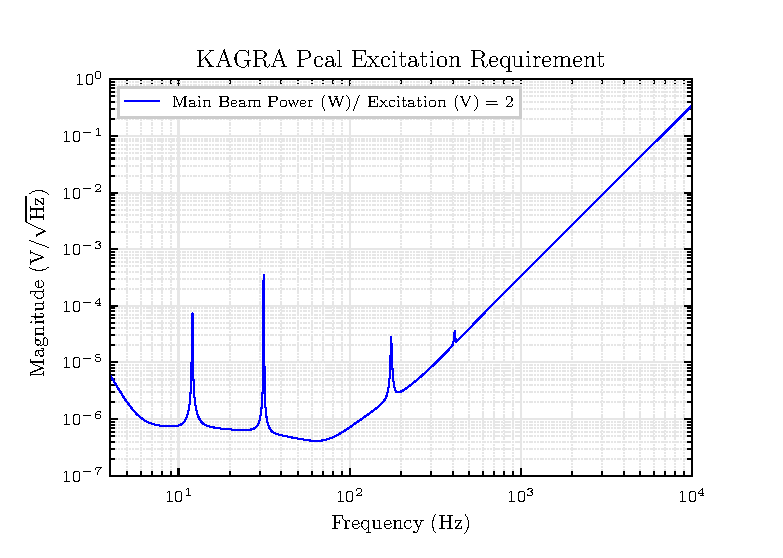
\includegraphics[width=.9\textwidth]{figure/DAC_requirement.eps}
\caption{Injection Channel Noise Requirement}\label{fig:DAC_noise_requirement}
\index{figures}
\end{figure}

\begin{align}
%\label{eq:}
   \Delta L(f) &< \frac{1}{10} \times (\text{KAGRA length sensitivity})\\
   \Delta L(f) =\frac{2 \Delta P(f) \cos(\theta)}{c} \frac{1}{M(2 \pi f)^2} &< \frac{1}{10} \Delta h(f) L
\end{align}








\section{Noise Source of Excitation channel}
\subsection{Quantization Noise of DAC}


The origin of quantization error is coming from the difference between desired analog output and quantized Digital to Analog Converter(DAC) output value. Roughly speaking, it shows like white noise spreading from DC to Nyquist frequency i.e. $Fs/2$.
The Root Mean Square value of quantization noise has the order of voltage difference corresponding to last digit or Least Significant Bit(LSB). In time domain, we can calculate standard deviation.
\begin{align}
%\label{eq:}
   \sigma_x = \sqrt{\frac{1}{12}} \delta x_{LSB}
\end{align}

For a 16-bit 64kHz DAC with output range between $\pm 10$Volts, 
\begin{align}
%\label{eq:}
    \sigma_x &= \sqrt{\frac{1}{12}} \delta x_{LSB} \\
             &= \sqrt{\frac{1}{12}} \frac{(+10)-(-10) \mathrm{Volts}}{2^{16}} \\
             &= 8.81 \times 10^{-5} \;\mathrm{Volts}
\end{align}

In frequency Domain, the quantization noise is distributed from DC to 32768Hz; therefore, we have ASD
\begin{align}
%\label{eq:}
    ASD &= \sqrt{PSD} \\
        &= \sqrt{ \frac{\sigma_x^2}{32768} } \\
        &= 8.81 \times 10^{-5} \sqrt{\frac{1}{32768}} \\
        &= 4.87 \times 10^{-7} \;\mathrm{Volts}/\sqrt{\mathrm{Hz}} 
\end{align}





\section{Noise Reduction through de-whitening filter}
Problem of 16kHz excitation channel 
Implementation of 64kHz Excitation channel in KAGRA digital system

Principle of Analog filter
Design of De-Whitening filter
Performance test
Transfer function measurement 
Noise requirement
Create Inverse De-Whitening filter


\chapter{Validation of Injection Channel}
Noise measurement
around 100Hz  the nose should below the IFO sensitivity
Transfer Function measurement
“above 1kHz” performance
time delay of excitation channel
(absolute timing measurement?)
Distortion of Scientific Signal
BBH
BNS post merger









































\chapter{Template}
Start off all chapters with \verb|chapter|. \index{chapter!numbered} \verb|\extrachapter| will give you an unnumbered chapter that's added to the Table of Contents. \index{chapter!unnumbered}

Here's an example of a citation \citep{GMP81}. Here's another \citep{PP98}. These will appear in the big bibliography at the end of the thesis.
\index{bibliography}

If you're new to \LaTeX{} and would like to begin by learning the basics, please see our free online course available at:\\ \url{https://www.overleaf.com/latex/learn/free-online-introduction-to-latex-part-1} \index{LaTeX@\LaTeX}

You can define nomenclatures \index{nomenclature} as you talk about key terms in your thesis. So what's a galaxy? \nomenclature{Galaxy}{A system of stars independent from all other systems}


\section{This is a Section}

\begin{figure}[hbt!]
\centering

\includegraphics[width=.3\textwidth]{NTNU.png}
\caption{This is a figure}\label{fig:logo}
\index{figures}
\end{figure}

\subsection{This is a subsection}

\begin{table}[hbt!]
\centering
\begin{tabular}{ll}
\hline
Area & Count\\
\hline
North & 100\\
South & 200\\
East & 80\\
West & 140\\
\hline
\end{tabular}
\caption{This is a table}\label{tab:sample}
\index{tables}
\end{table}

 \nomenclature{Asteroid}{A very small planet ranging from 1,000 km to less than one km in diameter. Asteroids are found commonly around other larger planets}



Here's an endnote.\endnote{Endnotes are notes that you can use to explain text in a document.}

\section{This is Another Section}



\printbibliography[heading=bibintoc]

\appendix
\printindex
\theendnotes

%% Pocket materials at the VERY END of thesis
%\pocketmaterial
%\extrachapter{Pocket Material: Map of Case Study Solar Systems} 


\end{document}
